%  Copyright 2020-2022 Robert Bosch GmbH
%
%  Licensed under the Apache License, Version 2.0 (the "License");
%  you may not use this file except in compliance with the License.
%  You may obtain a copy of the License at
%
%      http://www.apache.org/licenses/LICENSE-2.0
%
%  Unless required by applicable law or agreed to in writing, software
%  distributed under the License is distributed on an "AS IS" BASIS,
%  WITHOUT WARRANTIES OR CONDITIONS OF ANY KIND, either express or implied.
%  See the License for the specific language governing permissions and
%  limitations under the License.
\chapter{Code analysis}

The Robotframework AIO installation provides a static code analysis to detect potential errors and violations to coding conventions.
The name of the analyser is \textquotedbl{}Robocop\textquotedbl{}.

Start Eclipse and select a file or a folder in Project Explorer. A missing selection causes an error.

The External Tools menu provides three preconfigured settings to start the analysis (the numbering within the context menu
depends on the overall number of External Tools within your Eclipse configuration).

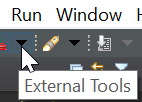
\includegraphics{./include/graphics/code_analysis/ExternalTools}

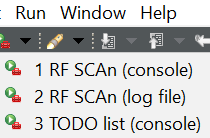
\includegraphics{./include/graphics/code_analysis/ContextMenu}

RF SCAn is the abbreviation for \textquotedbl{}\textbf{R}obot \textbf{F}ramework \textbf{S}tatic \textbf{C}ode \textbf{An}alysis\textquotedbl{}.

\textbf{1. RF SCAn (console)}
\begin{quote}
Output printed to console
\end{quote}

\textbf{2. RF SCAn (log file)}
\begin{quote}
Output printed to log file: \texttt{\%ROBOTLOGPATH\%\textbackslash{}Robocop.log}
\end{quote}

\textbf{3. TODO list (console)}
\begin{quote}
It is possible to use the string \texttt{TODO} in code comments to indicate that still something is \emph{todo}. But before a release all todo's should be resolved
(except there is a good and documented reason to keep the marker).
The static code analyser can be used to provide a list of all positions within your code, at which still such a \texttt{TODO} marker is present.
\end{quote}

\emph{Hint: The console displays a warning regarding rule '0906'. This warning can be ignored.}


